\documentclass[french, 12pt]{article}

\usepackage{geometry}
 \geometry{
 a4paper,
 total={150mm,240mm},
 left=30mm,
 top=30mm,
 }


\usepackage{helvet}

\usepackage[utf8]{inputenc}
\usepackage[T1]{fontenc}
\usepackage[french]{babel}
\usepackage{comment}
\usepackage{subcaption}
\usepackage{subfiles}
\usepackage{graphicx}
\usepackage{diagbox}
\usepackage[table,xcdraw]{xcolor}
% \usepackage{minted}
\usepackage{placeins}

\usepackage{fancyhdr}

% \setcounter{secnumdepth}{5}

\graphicspath{ {./img/} }

\title{\fontfamily{phv}\selectfont \Huge \textbf{Panic At Tortuga}}
\author{\fontfamily{phv}\Huge{Rapport de soutenance n°1}}
\date{\fontfamily{phv}\selectfont Février 2021}

\begin{document}

\begin{titlepage}
    \maketitle
    
    \thispagestyle{empty}
    % {\fontencoding{T1}\fontfamily{calligra}\selectfont the font is temporarily changed}
    \vspace{20pt}
    \begin{figure}[hbt!]
        \centering
        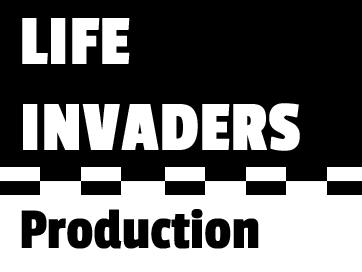
\includegraphics[scale=0.7]{logo_lifeinvaders_copie.png}
    \end{figure}
\end{titlepage}

% ////////////////////////////////////////////////
% ////////////////////////////////////////////////
% ////////////////////////////////////////////////


\tableofcontents
\newpage

\pagestyle{fancy}
\lhead{Panic At Tortuaga}
\fancyhead[C]{Février 2021}
\rhead{LifeInvaders Production}

\section{Introduction}

Panic At Tortuga est un jeu orienté multijoueur. Mais quel genre de est-ce ?
Il s'agit du jeu s'inspirant de mécaniques de jeux divers, 
les principaux étant Assassin's Creed (son mode multi) et d'autres jeux comme "Guess Who?".

Vous et d'autres joueurs êtes lachés sur la petite île de Tortuga, une île où la population vit paisiblement.
Mais parmi eux, déguisés, se cachent des pirates sanguinaires, et c'est à vous de les éliminer.

Le début de production de notre équipe de dévellopement, Lifeinvaders Production,
composé de Paul, Harrys, Julien et Dov; a pu commencer à développer le jeu depuis mi-décembre.
Nous avons pu apprendre de nombreuses choses, se dépaser, sortir de notre zone de confort, mais surtout prendre du plaisir à créer notre jeu !

% ////////////////////////////////////////////////
% ////////////////////////////////////////////////
% ////////////////////////////////////////////////

\section{Conception}

    Le concept de notre jeu se base sur une idée simple : Vous avez une cible et êtes celle d'un autre joueur.
    Vous devez éliminer chaque cible attribué (en l'occurence d'autres joueurs) et tenter de survivre dans ce petit archipel.

    Nous nous sommes répartis les taches rapidement les différentes tâches pour avoir les bases.
    Par exemple, le déplacement du personnage et de la caméra était primordial pour Harrys et Julien qui s'occupaient du multijoueur et nécéssitait d'être livré rapidement.
    Pendant que Renaud-Dov réalisait l'implémentation de ces scripts, Julien et Harrys ont commencé à apprendre comment fonctionnait Photon. Paul s'occupait alors de la map.

    Pour éviter de se perdre dans l'afflu de tâches à réaliser, nous décidé d'utiliser des outils de travail en équipe tel que des kanban (avec Github Projects).\\
    
    % Photo du kanban

    \begin{figure}[hbt!]
        \centering
        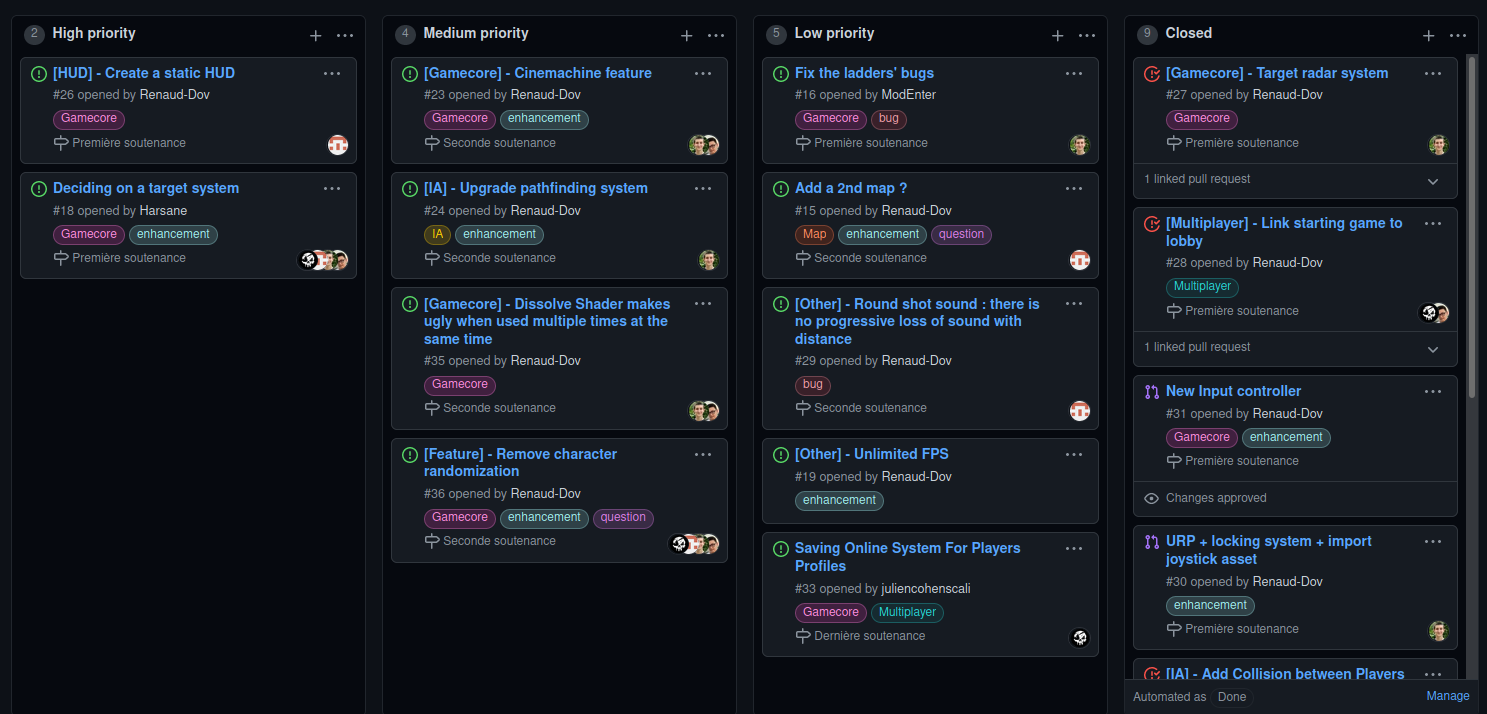
\includegraphics[scale=0.28]{kanban.png}
        \caption{Kanban pour la priorisation des tâches sur Github}
    \end{figure}


    \textbf{Tableau avec la répartition des tâches}

    % ////////////////////////////////////////////////
    % ////////////////////////////////////////////////
    % ////////////////////////////////////////////////
    
    \subsection{Réseau}

    % ////////////////////////////////////////////////
    % ////////////////////////////////////////////////
    % ////////////////////////////////////////////////

    \subsection{Intelligence Artificielle et NPC}

    Pour rendre notre jeu plus vivant et permettre aux joueurs de se méler dans la foule,
    il nous fallait créer des IA se déplacant dans la ville.
    Pour cela, nous avons décider d'utiliser des NavMesh pour créer des zones où les 
    NPC peuvent se balader d'un point A vers un point B.
    Pour ne pas rendre leur comportement linéaire et sans saveur,
    ils se déplacent de manière aléatoire  vers un point quelconque défini dans une liste de coordonées.
    Aucun NPC n'aura donc le même trajet.\\

    Pour rendre ces IA plus humaines, les joueurs peuvent les bousculer et les étourdir en courant vers eux.
    Ils reprenent leur trajet au bout de quelques secondes.


    Plusieurs problèmes se posent actuellement avec l'utilisation des NavMesh:
    \begin{itemize}
        \item L'IA calcule le chemin le plus court, et n'essaie pas de se déplacer sur le côté si d'autres IA marchent dans le sens contraire. Par exemple, si l'ont met deux escaliers cote à côte, toutes les IA vont prendre l'escalier le plus proche et donc se bloquer.\\
        \begin{figure}[hbt!]
            \centering
            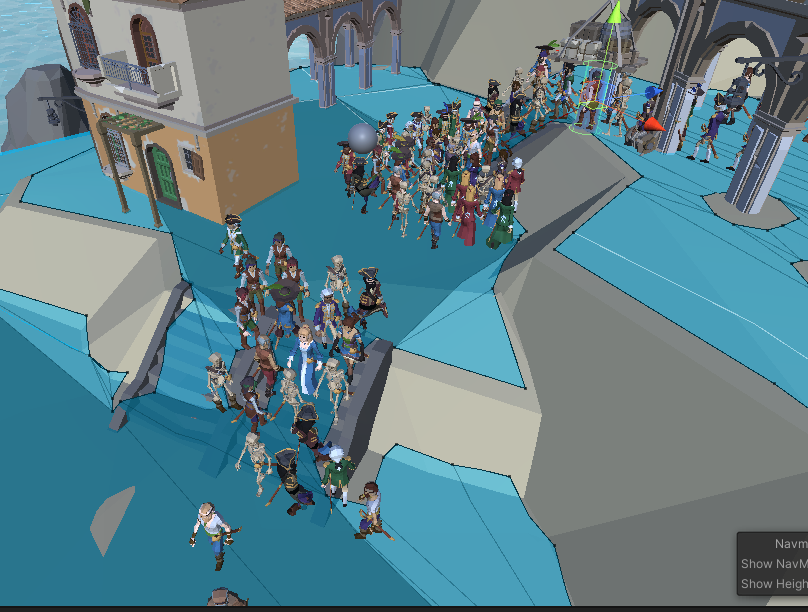
\includegraphics[scale=0.5]{ia_stairs_bug.png}
            \caption{Porte fermée après le passage d'un joueur}
        \end{figure}
    \end{itemize}

    % ////////////////////////////////////////////////
    % ////////////////////////////////////////////////
    % ////////////////////////////////////////////////

    \subsection{Mécaniques de jeu}

        \subsubsection{Environement}
            Nous nous sommes beaucoup inspiré du mode multijoueur des premiers Assassin's Creed.
            Nous n'avons pu récréer un système de grimpe car trop ardu à réaliser de nos propres mains.
            En revanche, nous avons réutilisé quelques idées de gameplay pour l'environement, comme les échelles et les portes.\\

            \begin{figure}[hbt!]
                \centering
                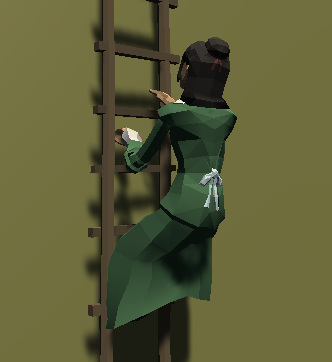
\includegraphics{ladder.png}
                \caption{Joueur grimpant sur l'échelle}
            \end{figure}

            L'échelle permet de créer un peu de verticalité dans nos niveaux.
            Elles ne peuvent être utilisées que par les joueurs,
            prendre de la hauteur permet d'emprunter des raccourcis, mais retire la discrétion (car personne de civilisé devrait être sur les toits !) \\
            
            Les portes peuvent vous permettre de barrer le passage pour échapper à son tueur. Elles se ferment quand le joueur passe dessus en courant,
            et se réouvrent au bout de quelques secondes.

            \begin{figure}[hbt!]
                \centering
                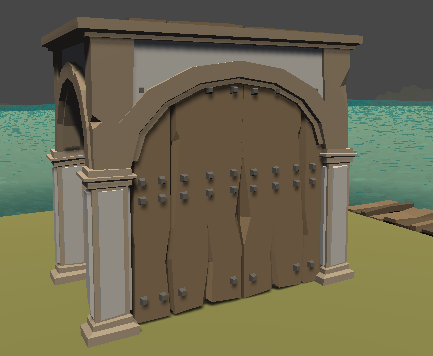
\includegraphics{doors_closed.png}
                \caption{Porte fermée après le passage d'un joueur}
            \end{figure}

        \subsection{Déplacement du personnage}
        
            Sans déplacement du personnage, le jeu serait ennuyeux si on ne pouvait interragir avec.
            Nous avons donc réalisé un script de déplacement qui permet au joueur de marcher, courir, sauter\dots\\

            Pour le côté technique, nous avons dans un premier temps utilisé l'Input System de base proposé par Unity. Mais plusieurs problèmes se sont posés:
            \begin{itemize}
                \item On ne peut paramétrer en profondeur les keymaps
                \item Paramétrer d'autres périphériques autre que le clavier/souris est compliqué. Il faudrait avoir des scripts différents pour chaque périphérique, et donc des prefabs différents
            \end{itemize}
            C'est pour cette raison que nous avons migré vers le New Input System.
            Celui ci est ergonomique, multiplateform et permet un mix de différents périphériques à fois, comme la manette par exemple.
            Il a fallu editer certains bout de code pour les rendre compatible; heureusement, la migration ne fut pas très longue après avoir compris son fonctionnement.

            Il est donc actuellement possible de jouer au clavier/souris ou à la manette (pas les deux à fois).
        
        \subsection{Système de verrouilage}

            Le système qui attribue des cibles à chaque joueur n'est pas entièrement implémenté.
            
            Mais le joueur peut vouloir tuer une cible, qu'elle soit la bonne ou non.
            Pour cela, il passe en mode verrouilage, et les personnages pointés par le viseur surbrillent.
            Pour les sélectionner, un coup de molette suffit, et le contour devient alors jaune, pour indiquer que la cible est verouillé.
            Il lui suffit alors d'être à moins d'1 mètre pour l'éliminer.

            \begin{figure}[hbt!]
                \centering
                \begin{subfigure}[b]{0.3\textwidth}
                    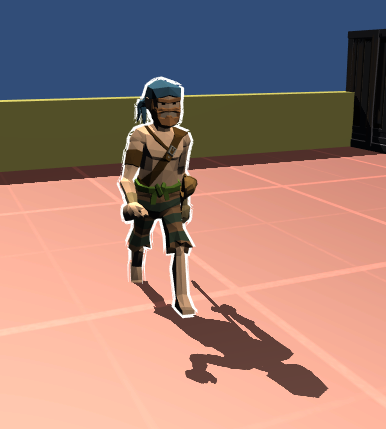
\includegraphics[scale=0.1]{white_outline.png} 
                    \caption{}
                \end{subfigure}
                \hspace{150pt}
                \begin{subfigure}[b]{0.3\textwidth}
                    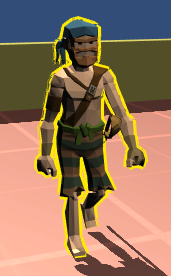
\includegraphics[scale=0.5]{yellow_outline.png} 
                    \caption{Animation de course sur un personnage}
                \end{subfigure}
                \caption{Animations de Mixamo vers Unity}
            \end{figure}


    % ////////////////////////////////////////////////
    % ////////////////////////////////////////////////
    % ////////////////////////////////////////////////
    
    \subsection{Menus : HUD/Menus}

    % ////////////////////////////////////////////////
    % ////////////////////////////////////////////////
    % //////////////////////////////////////////////// 

    \subsection{Carte du jeu}

    Pour la partie graphique, nous n'avons pas choisi de réaliser
    nous-même les textures et autres meshes pour notre jeu.
    Nous avons plutôt opté pour un asset payant,
    nous permettant de nous focaliser plus sur les mécaniques de jeu et l'implémentation
    du multijoueur.

% ////////////////////////////////////////////////
% ////////////////////////////////////////////////
% ////////////////////////////////////////////////

\section{Avance et retard}

% ////////////////////////////////////////////////
% ////////////////////////////////////////////////
% ////////////////////////////////////////////////
\section{Prévisions}
% ////////////////////////////////////////////////
% ////////////////////////////////////////////////
% ////////////////////////////////////////////////

\end{document}
